\RequirePackage{atbegshi}
\documentclass[compress]{beamer}

\usepackage{graphicx,epstopdf,subfigure,booktabs,natbib}
\usepackage{tikz}
\usetikzlibrary{positioning,arrows,shapes}

%\usetheme[compress,subsection=F]{Singapore}
%\useoutertheme[subsection=false]{miniframes}
\usetheme[hideallsubsections]{Hannover}
%\usecolortheme{dove}
\usecolortheme{seagull}
\useinnertheme{default}

\bibliographystyle{plainnat}
\bibpunct{[}{]}{;}{a}{}{,}
\usefonttheme{serif}
\usepackage{mathpazo}
\pgfrealjobname{bracken-crbhwg-2009}

\title[Interannual Scale]{Reclamation Review of Stochastic Streamflow Simulation at Interannual and Interdecadal Time Scales and Implications to Water Resources Management}
\subtitle{Past, Present and Future Work}
\author[Cameron Bracken]{Cameron Bracken\\CADSWES, CU Boulder}
\date{October 5th, 2009}

\begin{document}

%%%%%%%%%%%%%%%%%%%%%%%%%%%%%%%%%%%%%%%%%%%%%%%%%%%%%%
%%%%%%%%%%%%%%%%%%%%%%%%%%%%%%%%%%%%%%%%%%%%%%%%%%%%%%
\begin{frame}
\titlepage
\end{frame}


%%%%%%%%%%%%%%%%%%%%%%%%%%%%%%%%%%%%%%%%%%%%%%%%%%%%%%
%%%%%%%%%%%%%%%%%%%%%%%%%%%%%%%%%%%%%%%%%%%%%%%%%%%%%%
\section{Background}
\subsection{Background}
\begin{frame}{Background}
\begin{itemize}
\item Research Experience for Undergraduates, Summer 2007
\item B.S. Environmental Resources Engineering / Applied Math, Humboldt State University, 2009
\item CADSWES Summer 2009
\item Started CU Boulder Civil Engineering MS program Fall 2009
\end{itemize}
\end{frame}


%%%%%%%%%%%%%%%%%%%%%%%%%%%%%%%%%%%%%%%%%%%%%%%%%%%%%%
%%%%%%%%%%%%%%%%%%%%%%%%%%%%%%%%%%%%%%%%%%%%%%%%%%%%%%
\section{Past Work}
\subsection{REU Project}
\begin{frame}{Past Work - REU Project}
\pause
The goal of the project was to: 
\begin{itemize}
  \item Develop a \alert{seasonal streamflow forecast framework}
\begin{itemize}

\item Handle many spatial locations 
\item Preserve spatial and temporal dependencies
\item Incorporate large scale climate predictors
\item Use modern nonparametric methods
\item Generate multi-model ensembles
\end{itemize}
\end{itemize}


\end{frame}

%%%%%%%%%%%%%%%%%%%%%%%%%%%%%%%%%%%%%%%%%%%%%%%%%%%%%%
%%%%%%%%%%%%%%%%%%%%%%%%%%%%%%%%%%%%%%%%%%%%%%%%%%%%%%
\subsection{Seasonal Flow Forecast Framework}
\begin{frame}{Past Work - Findings}
%\beginpgfgraphicnamed{figs/framework}
%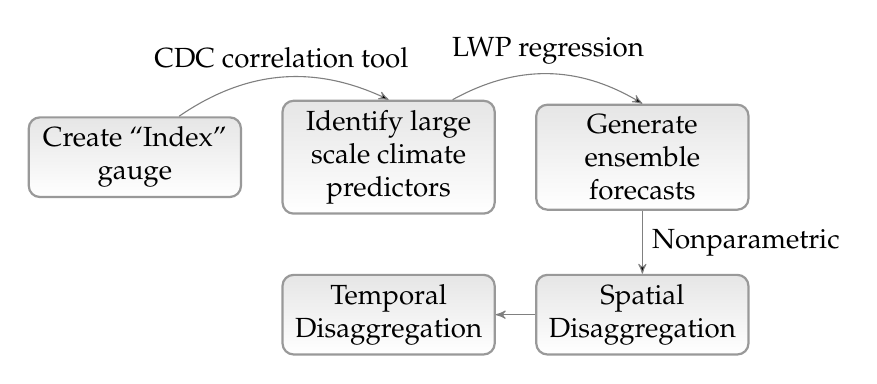
\begin{tikzpicture}
    [
    node distance=8mm and 5mm,
    block/.style ={
        rectangle, 
        draw=gray!80, 
        thick, 
        top color=gray!20, 
        bottom color=white,
        text badly centered, 
        text width=7em,
        rounded corners
    },
    a/.style={
        -stealth',
        draw=gray
    }
    ]
    \node (index)[block] {Create ``Index'' gauge};
    \node (predictors)[block,right=of index] {Identify large scale climate predictors};
    \node (ensemble)[block,right=of predictors] {Generate ensemble forecasts};
    \node (spatial)[block,below=of ensemble] {Spatial Disaggregation};
    \node (temporal)[block,left=of spatial] {Temporal Disaggregation};
      
    \draw[a] (index) edge [bend left] node [above] {CDC correlation tool} (predictors.90);
    \draw[a] (predictors) edge [bend left] node [above] {LWP regression} (ensemble.90);
    \draw[a] (ensemble) edge node [right] {Nonparametric} (spatial);
    \draw[a] (spatial) -- (temporal);
    
\end{tikzpicture}

%\endpgfgraphicnamed
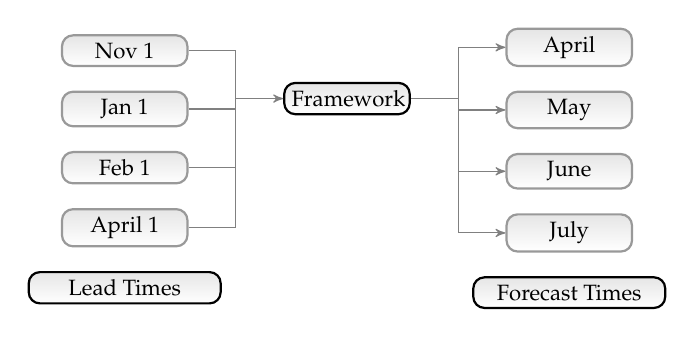
\begin{tikzpicture}
    [
    node distance=3mm and 5mm,
    block/.style ={
        rectangle, 
        draw=gray!80, 
        thick, 
        top color=gray!20, 
        bottom color=white,
        text badly centered, 
        text width=5em,
        rounded corners
    },
    phantom/.style={
        inner sep=0,
        outer sep=-.7pt,
    },
    a/.style={
        -stealth',
        draw=gray
    },
    l/.style={
        draw=gray
    }
    ]
    \footnotesize
    \node (lead1)[block] {Nov 1};
    \node (lead2)[block,below=of lead1] {Jan 1};
    \node (lead3)[block,below=of lead2] {Feb 1};
    \node (lead4)[block,below=of lead3] {April 1};
    \node (leaddes)[block,draw=black,text width=8em,below=of lead4] {Lead Times};
    
    \node (p1)[below right=of lead1]{};
    
    \node (f)[block,right=of p1,draw=black] {Framework};
    
    \node (p2)[right=of f]{};
    
    \node (fc1)[block,above right=of p2] {April};
    \node (fc2)[block,below=of fc1] {May};
    \node (fc3)[block,below=of fc2] {June};
    \node (fc4)[block,below=of fc3] {July};
    \node (fcdes)[block,draw=black,text width=8em,below=of fc4] {Forecast Times};
      
    \draw[l] (lead1) -| (p1.center);
    \draw[l] (lead2) -| (p1.center);
    \draw[l] (lead3) -| (p1.center);
    \draw[l] (lead4) -| (p1.center);
    
    \draw[a] (p1.center) -- (f);
    
    \draw[a] (p2.center) |- (fc1);
    \draw[a] (p2.center) |- (fc2);
    \draw[a] (p2.center) |- (fc3);
    \draw[a] (p2.center) |- (fc4);
    
    \draw[l] (p2.center) -- (f);
    
\end{tikzpicture}

\begin{figure}[htbp]
   \centering
   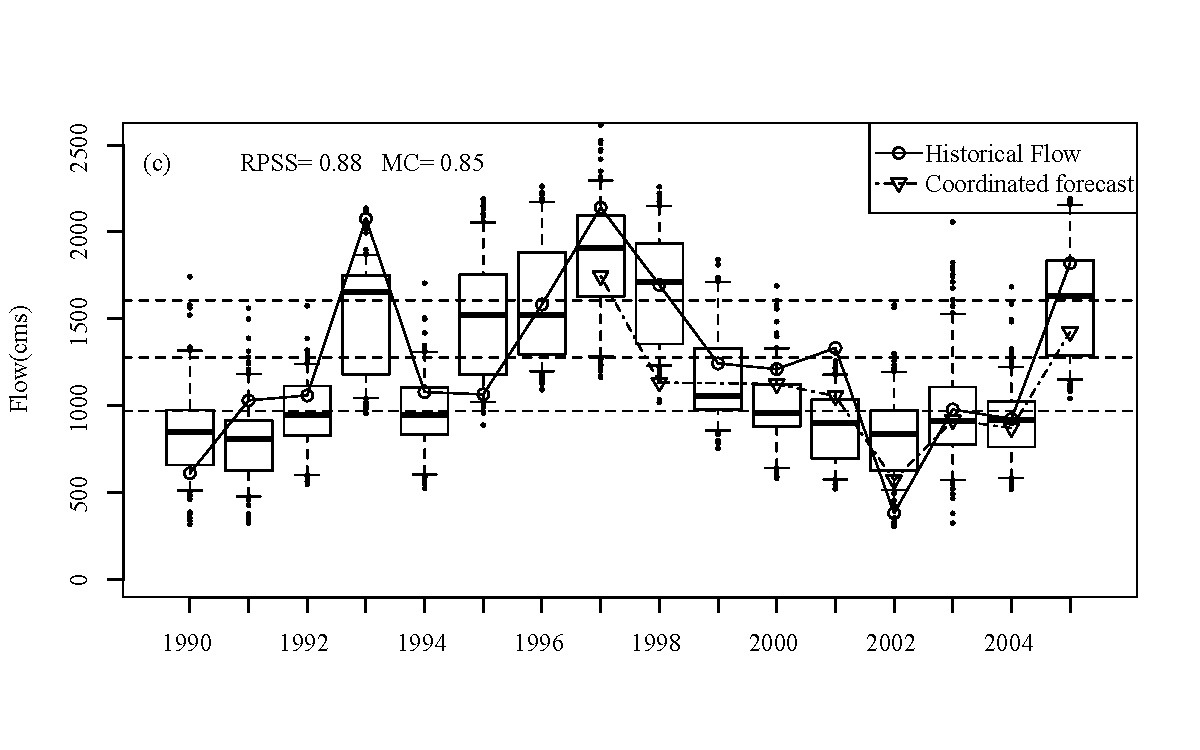
\includegraphics[width=.9\textwidth]{figs/figure-9b.pdf} 
   %\caption{Seasonal flows at Lees Ferry}
\end{figure}


\begin{itemize}
\item Results are a ``proof-of-concept.''
\item Forecast skill is retained after disag.
\item A relatively simple, robust framework that compares well to existing models.
\end{itemize}

%\pause
%Bracken, C., B. Rajagopalan, J. Prairie (2009), A multi-site seasonal ensemble streamflow forecasting technique, {\it Water Resources Research}, In Review.
\end{frame}

%%%%%%%%%%%%%%%%%%%%%%%%%%%%%%%%%%%%%%%%%%%%%%%%%%%%%%
%%%%%%%%%%%%%%%%%%%%%%%%%%%%%%%%%%%%%%%%%%%%%%%%%%%%%%
\section{Current Work}
\subsection{Probabilistic Midterm Model}
\begin{frame}{Current and Future Work}
\framesubtitle{Probabilistic Midterm Model}
\pause
\begin{itemize}
\item Midterm operational forecast model for the CRB
\item Next generation 24 month study
\item New features
	\begin{itemize}
	\item Multiple traces
	\item Second year forecasts
	\item Demands 
	\item Operational rules
	\item Real time data inputs
	\end{itemize}
\end{itemize}

\end{frame}

\subsection{Groundwork for PMM - Natural Flow Comparisons}
\begin{frame}{Groundwork for the PMM}
\framesubtitle{Natural Flow Comparisons}
\begin{itemize}
\item Attempt to understand the differences between the River Forecast Center's real time flows and Reclamation's natural flow.
	\begin{itemize}
		\item Start by plotting differences (6 sites)
	\end{itemize}
\end{itemize}
\pause
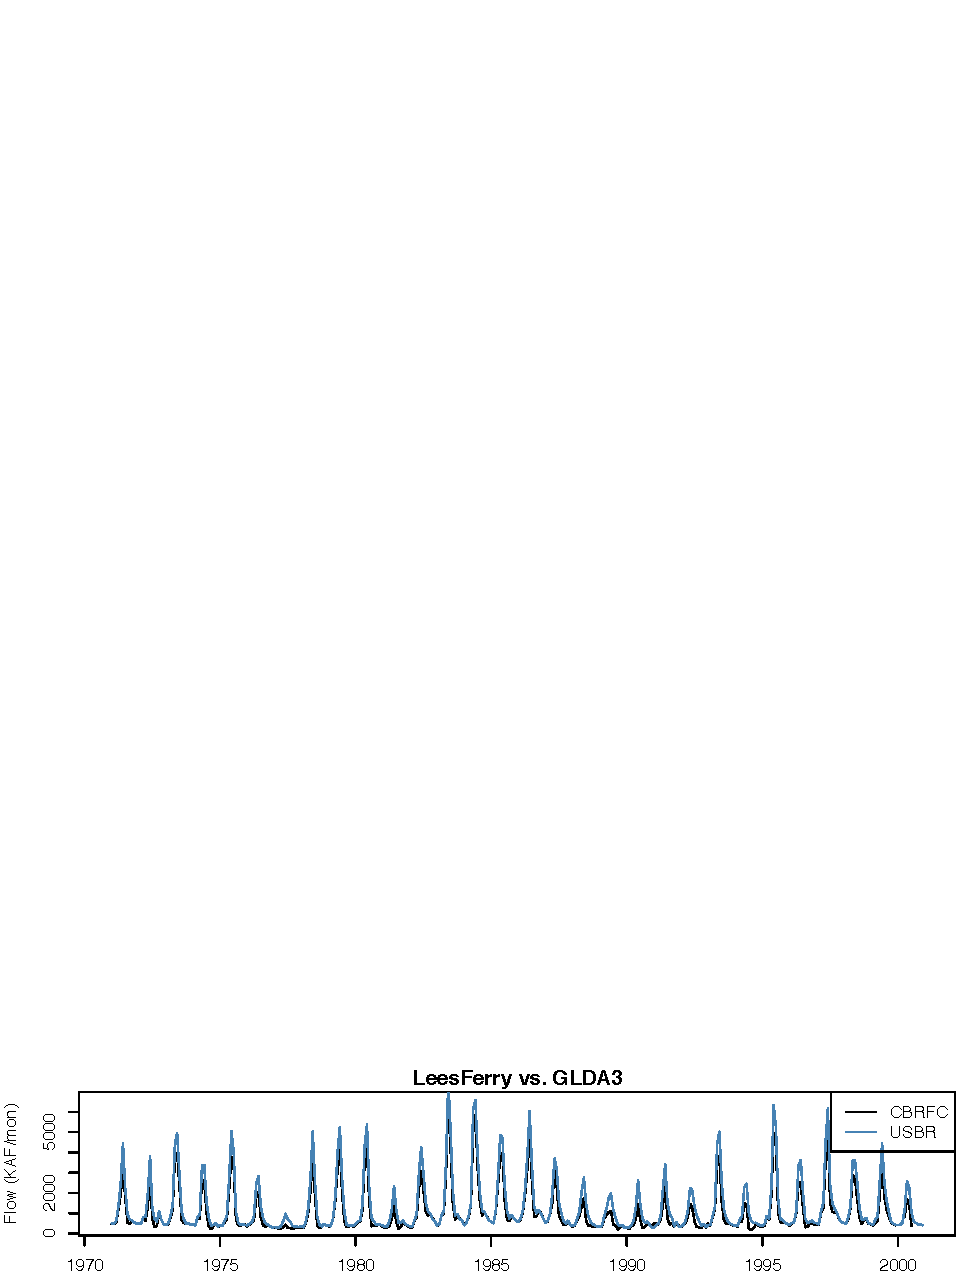
\includegraphics[width=\textwidth]{figs/lees-data.pdf}\\
\pause
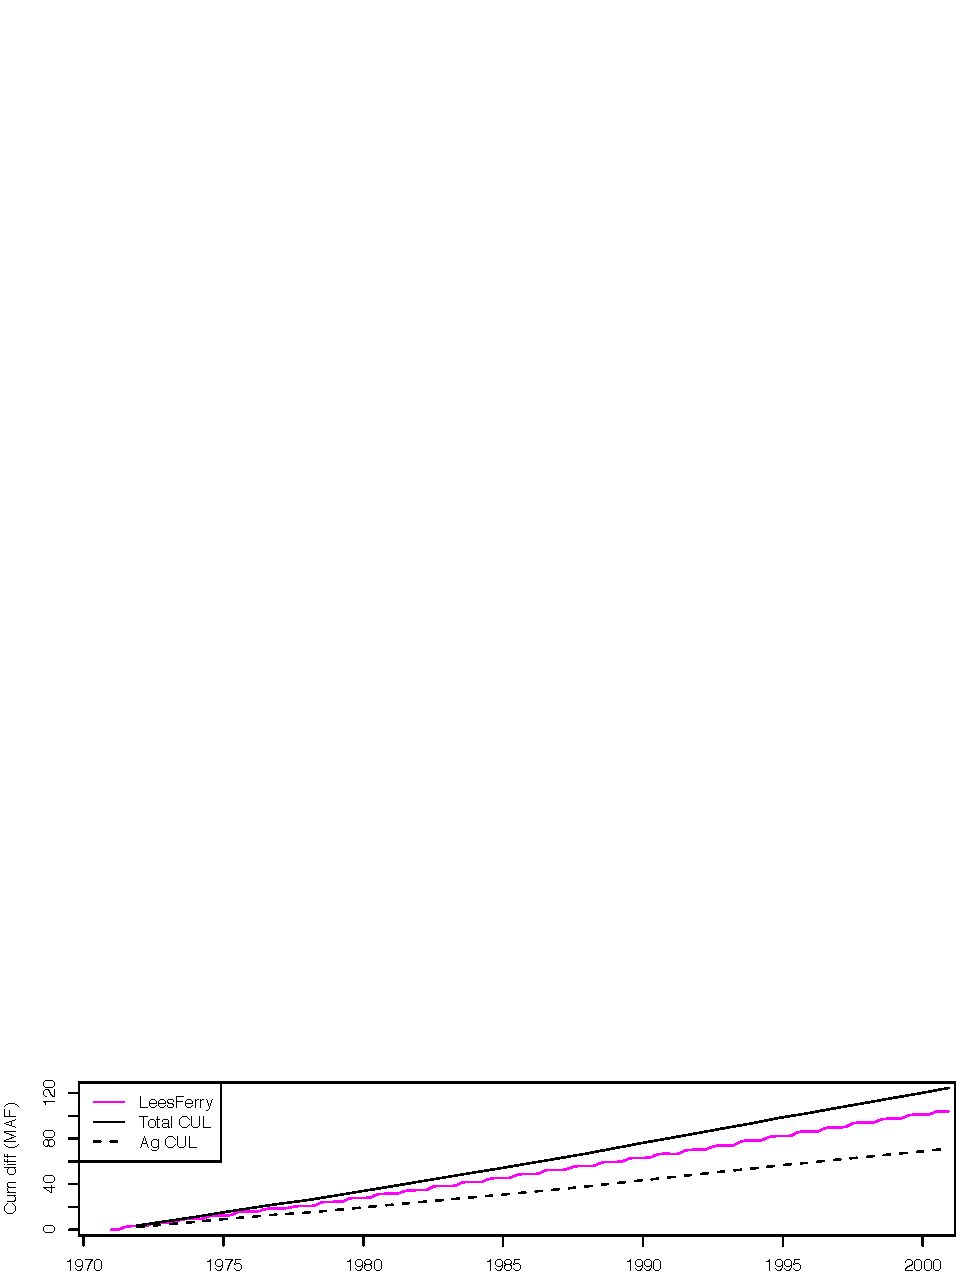
\includegraphics[width=\textwidth]{figs/cum-diff.pdf} 
\end{frame}

%%%%%%%%%%%%%%%%%%%%%%%%%%%%%%%%%%%%%%%%%%%%%%%%%%%%%%
%%%%%%%%%%%%%%%%%%%%%%%%%%%%%%%%%%%%%%%%%%%%%%%%%%%%%%
\subsection{Findings So Far}
\begin{frame}{Important results so far}
\begin{itemize}
	\item RFC data seems to be ``not quite'' unregulated.  
	\item Some fundamental modeling differences uncovered at Navajo (Archuletta).
\end{itemize}
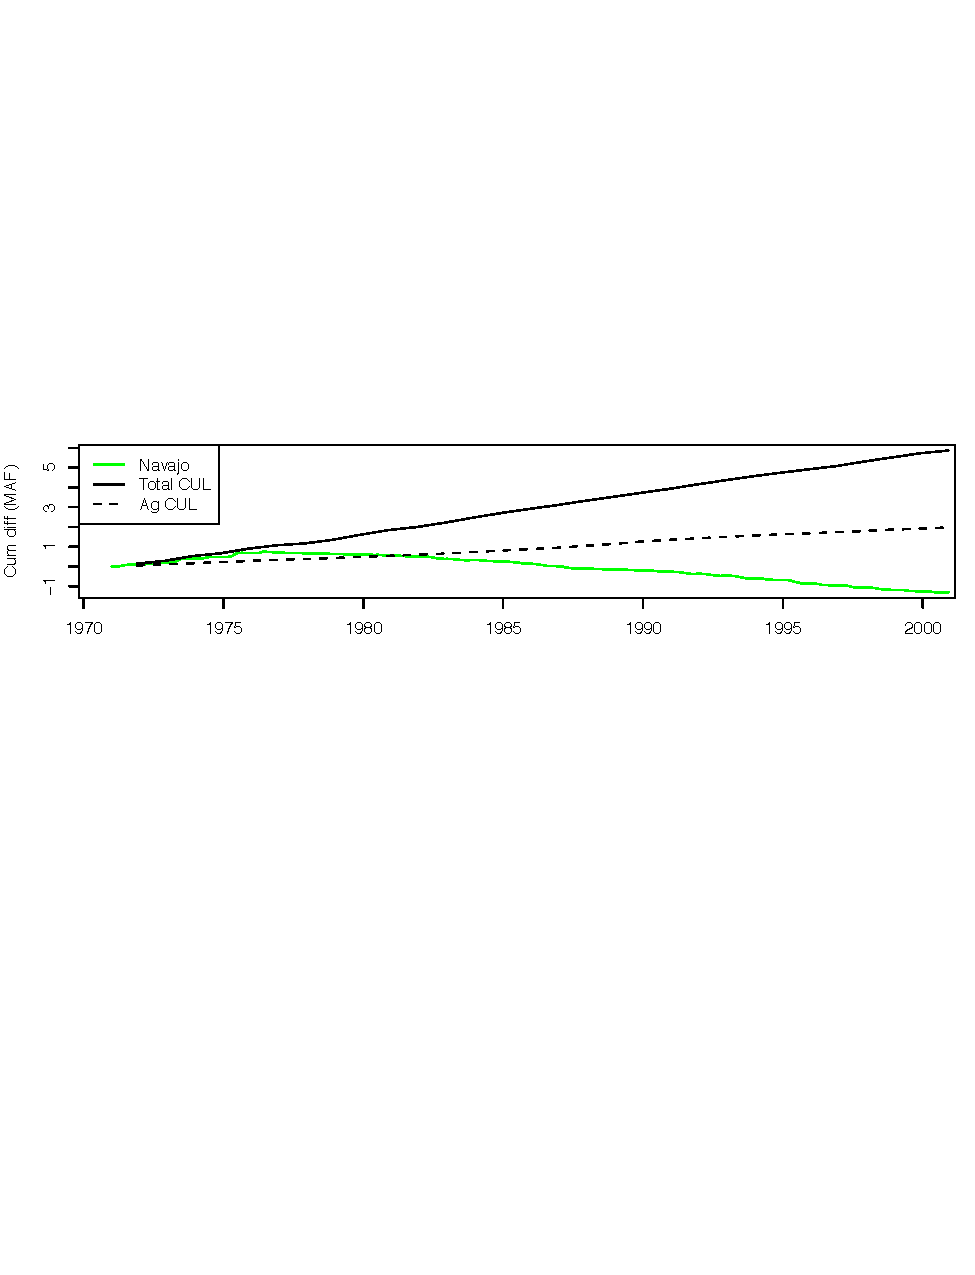
\includegraphics[width=\textwidth]{figs/cum-diff-navajo.pdf} 
\end{frame}

%%%%%%%%%%%%%%%%%%%%%%%%%%%%%%%%%%%%%%%%%%%%%%%%%%%%%%
%%%%%%%%%%%%%%%%%%%%%%%%%%%%%%%%%%%%%%%%%%%%%%%%%%%%%%
\section{Future Work}
\subsection{Probabilistic midterm model}
\begin{frame}{Next Steps}
\begin{itemize}
\item Continue to investigate RFC modeling differences
\item Operational rulesets for forecast points (Fontenelle)
\item Intelligent 2nd year seasonal forecasts
\end{itemize}
\end{frame}

\section{~}

\end{document}  